\documentclass{article}
\usepackage{caption}
\usepackage{subcaption}
\usepackage{graphicx}
\usepackage{tikz}
\usepackage{tikzsymbols}
\usetikzlibrary{calc}
\usepackage{float}
\usepackage{pdflscape}

\def\centerarc[#1](#2)(#3:#4:#5){\draw[#1] ($(#2)+({#5*cos(#3)},{#5*sin(#3)})$) arc (#3:#4:#5);}

\pagestyle{empty}
\begin{document}
	\centering
	\begin{figure}[H]
			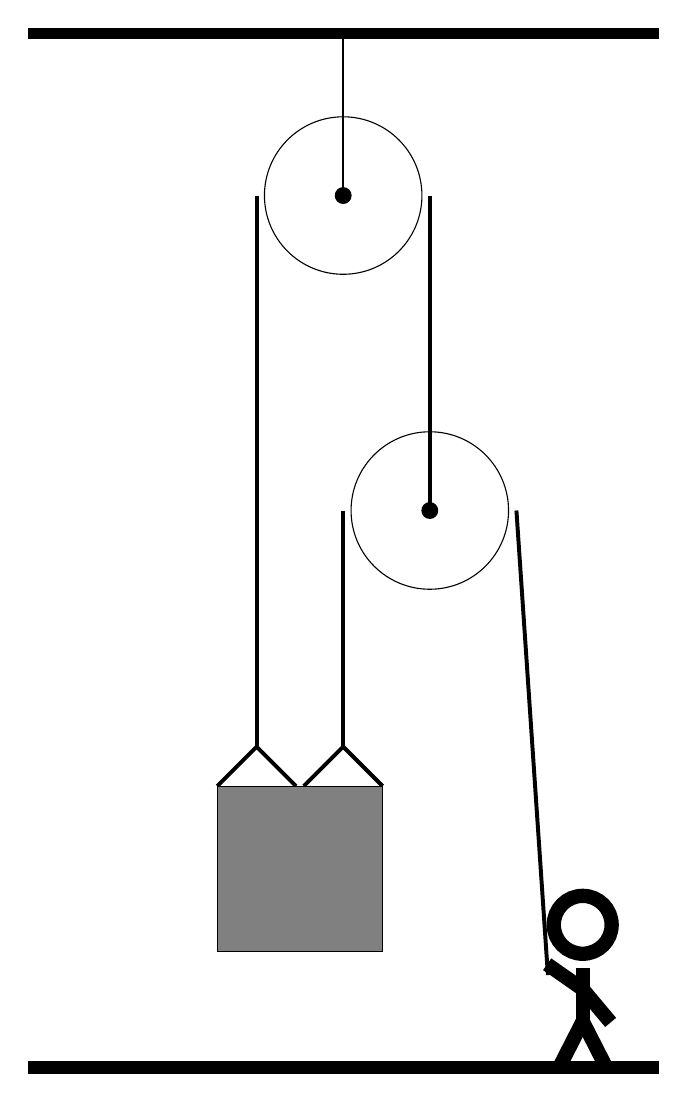
\begin{tikzpicture}
				%%%%% START %%%%%
				\def\a{10}
				\def\radlg{1}
				\def\radrp{1.1}
				\def\radsm{0.1}
				\def\xone{2}
				\def\yone{\a-\a*0.2}
				\def\xtwo{3.1}
				\def\ytwo{\a-\a*0.6}
				\def\dx{5}
				\def\dy{-2}
				\def\hlen{\a*0.9}
				\def\width{0.5mm}

				\draw[fill=black] (-2,\a) rectangle (6,\a+0.125);

				\draw (\xone,\yone) circle (\radlg);
				\draw[fill=black] (\xone,\yone) circle (\radsm);
				\draw[thick] (\xone,\yone) -- (\xone,\a);

				\draw (\xtwo,\ytwo) circle (\radlg);
				\draw[fill=black] (\xtwo,\ytwo) circle (\radsm);

				\draw[line width = \width]  (\xone-\radrp-0.5,\a-\hlen-0.5) -- (\xone-\radrp,\a-\hlen) -- (\xone-\radrp+0.5,\a-\hlen-0.5);
				\draw[line width = \width]  (\xtwo-\radrp-0.5,\a-\hlen-0.5) -- (\xtwo-\radrp,\a-\hlen) -- (\xtwo-\radrp+0.5,\a-\hlen-0.5);
				\draw[fill=black!50] (\xone-\radrp-0.5,\a-\hlen-0.5) rectangle (\xone-\radrp+1.6,\a-\hlen-0.5-2.1);

				\draw[line width = \width] (\xone-\radrp,\yone) -- (\xone-\radrp,\a-\hlen);
				\centerarc[line width = \width](\xone,\yone)(0:180:\radrp);
				\draw[line width = \width] (\xone+\radrp,\yone) -- (\xtwo,\ytwo);
				\draw[line width = \width] (\xtwo-\radrp,\ytwo) -- (\xtwo-\radrp,\a-\hlen);
				\centerarc[line width = \width](\xtwo,\ytwo)(0:180:\radrp);
				\draw[line width = \width] (\xtwo+\radrp,\ytwo) -- (\dx-0.4,\dy+0.1);

				\node at (\dx,\dy) {\Strichmaxerl[10][-35][-50]};
						
				\draw[fill=black] (-2,-3) rectangle (6,-3.15);
				%%%%% START %%%%%
			\end{tikzpicture}
	\end{figure}

\end{document}